\documentclass[10pt, letterpaper]{article}

\usepackage{tikz}
\usepackage{amsmath}
\usepackage{pgfplots}
\pgfplotsset{compat=1.9}
\usetikzlibrary{arrows,shapes,automata,backgrounds,petri,fit,decorations.pathmorphing, calc}

\begin{document}

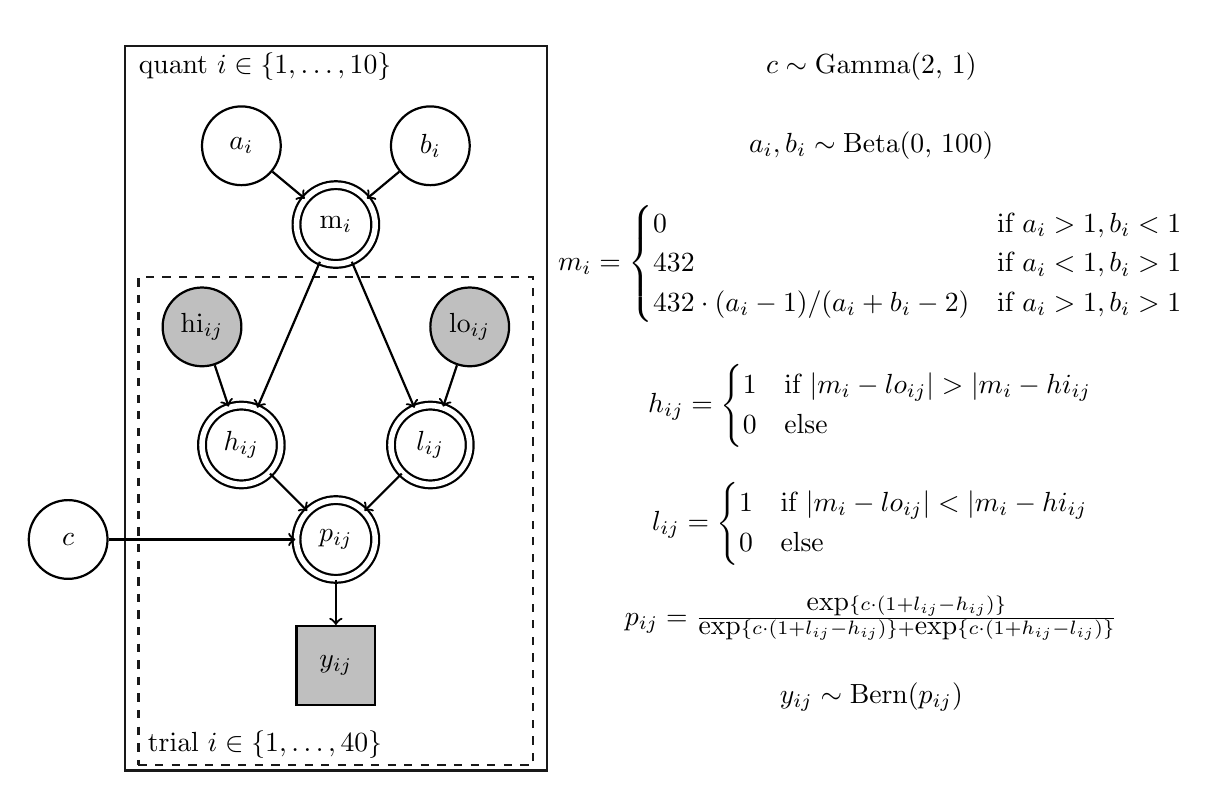
\begin{tikzpicture}[node distance = 2.4cm, double distance = 2pt, minimum size=1cm, thick]
  \node[circle, draw=black] (a) {$a_i$};
  \node[circle, draw=black, right of = a] (b) {$b_i$};
  
  \node[circle, double, draw=black, right of = a, below of = a, node distance = 1.2cm, yshift = .2cm]
  (m) {$\mbox{m}_i$};
  
  \node[circle, draw=black, below of = a, double, node distance = 3.8cm] (h) {$h_{ij}$};
  \node[circle, draw=black, right of = h, double] (l) {$l_{ij}$};
  
  \node[circle, draw=black, fill=lightgray, above of = h, node distance = 1.5cm, xshift = -.5cm]
  (hi) {$\mbox{hi}_{ij}$};
  \node[circle, draw=black, fill=lightgray, above of = l, node distance = 1.5cm, xshift = +.5cm] (lo)
  {$\mbox{lo}_{ij}$};
  
  \node[circle, draw=black, below of = h, right of = h, double, node distance = 1.2cm] (p) {$p_{ij}$};
  \node[circle, draw=black, left of = p, node distance = 3.4cm] (c) {$c$};
  
  \node[rectangle, draw=black, fill=lightgray, below of = p, node distance = 1.6cm] (y) {$y_{ij}$};
  
  \draw[->] (c)--(p);
  \draw[->] (a)--(m);
  \draw[->] (b)--(m);
  \draw[->] (m)--(h);
  \draw[->] (m)--(l);
  
  \draw[->] (hi)--(h);
  \draw[->] (lo)--(l);
  \draw[->] (h)--(p);
  \draw[->] (l)--(p);
  \draw[->] (p)--(y);
  
   \begin{pgfonlayer}{background}
       \node [thick,
              draw=black!90,fit={($(y.south)+(0,-20pt)$) 
                                 ($(hi.west)+(-10pt,-10pt)$) 
                                 ($(a.north)+(0,18pt)$) 
                                 ($(lo.east)+(+10pt,+10pt)$)}] {};
    \end{pgfonlayer}
    
    \node[above of = a, node distance = 1cm] (QuantAnchor) {};
    \node[right of = QuantAnchor, node distance = .3cm] (QuantLabel) {quant $i \in \{1, \ldots, 10\}$};
    
   \begin{pgfonlayer}{background}
       \node [thick, dashed,
              draw=black!90,fit={($(y.south)+(0,-18pt)$) 
                                 ($(hi.west)+(-5pt,-5pt)$) 
                                 ($(hi.north)+(0,0)$) 
                                 ($(lo.east)+(+5pt,+5pt)$)}] {};
    \end{pgfonlayer}
    
    \node[below of = y, node distance = 1cm] (TrialAnchor) {};
    \node[left of = TrialAnchor, node distance = .9cm] (TrialLabel) {trial $i \in \{1, \ldots, 40\}$};
  
  
    \begin{scope}[xshift = 8cm, node distance = 1cm]
  
        \node[] at(0,1) (c) {$c \sim \mbox{Gamma(2, 1)}$};
        \node[below of = c] (a) {$a_i, b_i \sim \mbox{Beta(0, 100)}$};
        
        \node[below of = a, node distance = 1.5cm] (m)
        {$m_i = \begin{cases}
                  0 & \text{if } a_i > 1, b_i < 1 \\
                  432 & \text{if } a_i < 1, b_i > 1 \\
                  432 \cdot (a_i - 1) / (a_i + b_i - 2) & \text{if } a_i > 1, b_i > 1 \\
                 \end{cases}$};
                 
        \node[below of = m, node distance = 1.8cm] (h)
        {$h_{ij} = \begin{cases}
                     1 & \text{if } |m_i - lo_{ij}| > |m_i - hi_{ij} \\
                     0 & \text {else}
                   \end{cases}$};
        
        \node[below of = h, node distance = 1.5cm] (l)
        {$l_{ij} = \begin{cases}
                     1 & \text{if } |m_i - lo_{ij}| < |m_i - hi_{ij} \\
                     0 & \text {else}
                   \end{cases}$};
  
        \node[below of = l, node distance = 1.2cm] (p)
        {$p_{ij} = \frac{\mbox{exp}\left\{ c \cdot (1 + l_{ij} - h_{ij}) \right\}}
        {\mbox{exp}\left \{c \cdot (1 + l_{ij} - h_{ij}) \right \} +
        \mbox{exp} \left \{ c \cdot (1 + h_{ij} - l_{ij}) \right \}}$};
        
        \node[below of = p] (yij) {$y_{ij} \sim \mbox{Bern(}p_{ij})$};
        
    \end{scope}
    
\end{tikzpicture}

\end{document}